\documentclass[8pt]{beamer}
% Created By Gouthaman KG
%~~~~~~~~~~~~~~~~~~~~~~~~~~~~~~~~~~~~~~~~~~~~~~~~~~~~~~~~~~~~~~~~~~~~~~~~~~~~~~
% Use roboto Font (recommended)
\usepackage[sfdefault]{roboto}
\usepackage[utf8]{inputenc}
\usepackage[T1]{fontenc}
\usepackage{adjustbox}
%~~~~~~~~~~~~~~~~~~~~~~~~~~~~~~~~~~~~~~~~~~~~~~~~~~~~~~~~~~~~~~~~~~~~~~~~~~~~~~

%~~~~~~~~~~~~~~~~~~~~~~~~~~~~~~~~~~~~~~~~~~~~~~~~~~~~~~~~~~~~~~~~~~~~~~~~~~~~~~
% Define where theme files are located. ('/styles')
\usepackage{styles/fluxmacros}
\usefolder{styles}
% Use Flux theme v0.1 beta
% Available style: asphalt, blue, red, green, gray 
\usetheme[style=asphalt]{flux}
%~~~~~~~~~~~~~~~~~~~~~~~~~~~~~~~~~~~~~~~~~~~~~~~~~~~~~~~~~~~~~~~~~~~~~~~~~~~~~~

%~~~~~~~~~~~~~~~~~~~~~~~~~~~~~~~~~~~~~~~~~~~~~~~~~~~~~~~~~~~~~~~~~~~~~~~~~~~~~~
% Extra packages for the demo:
\usepackage{booktabs}
\usepackage{colortbl}
\usepackage{ragged2e}
\usepackage{schemabloc}
\usepackage{hyperref}
\usebackgroundtemplate{

\includegraphics[width=\paperwidth,height=\paperheight]{assets/background.jpg}}%change this to your preferred background for the presentation.
%~~~~~~~~~~~~~~~~~~~~~~~~~~~~~~~~~~~~~~~~~~~~~~~~~~~~~~~~~~~~~~~~~~~~~~~~~~~~~~

%~~~~~~~~~~~~~~~~~~~~~~~~~~~~~~~~~~~~~~~~~~~~~~~~~~~~~~~~~~~~~~~~~~~~~~~~~~~~~~
% Informations
\title{MANAGING SUPPLY \\ IN THE INDIAN CONTEXT:
\\FLEXIBLE WORKERS, FULL-TIME EMPLOYEES AND FREELANCERS}

\author{Tanvi Ohri and Manne Hema Priya}
\institute{}
\titlegraphic{iitglogo.eps} %change this to your preferred logo or image(the image is located on the top right corner).
%~~~~~~~~~~~~~~~~~~~~~~~~~~~~~~~~~~~~~~~~~~~~~~~~~~~~~~~~~~~~~~~~~~~~~~~~~~~~~~

\begin{document}

% Generate title page
\titlepage

\begin{frame}

 \frametitle{TABLE OF CONTENTS}
 \tableofcontents
\end{frame}
\section{Introduction}
\begin{frame}{Introduction}
    The main aim of the project is to adapt the model proposed by Dong and Ibrahim (2020) \cite{dong} for the Indian market.There is a rise in the number of firms that are staffing a blended workforce. The model proposed in Dong and Ibrahim (2020) \cite{dong} considers two types of employees the fixed and flexible. With the increasing trend of startups in India, we feel we need to include another type of employee- the freelancer. The flexible employee is hired for a short interval, say when we typically expect higher traffic or a certain kind of work. The freelancers are hired for a particular task, that is, the profession's or startup's area of expertise. Our goal is to devise an optimal staffing strategy to the combat supply-side uncertainty which staffs freelancers, flexible workers and full-time employees. The strategy must take into account both quality and efficiency factors.
\end{frame}
\section{Brief of work done in phase 1}
\begin{frame}{Brief of work done in phase 1}
    In phase 1, we started out by understanding some basic ideas of queuing theory like newspaper vendor problem\cite{newsvendor} and square root staffing law. Then we examined optimal staffing under parameter uncertainty \cite{bassamboo} and optimal staffing using only flexible servers and no parameter uncertainty \cite{ibrahim}. In this phase, we will combine both these ideas and implement the model in Dong and Ibrahim (2020)\cite{dong} along with adding freelancers to the model, we also look at some numerical results.
\end{frame}
\section{Capacity sizing with only self scheduling servers}
\begin{frame}{Capacity sizing with only self scheduling servers}
    In this chapter we will look at a workforce consisting of only flexible i.e. self-scheduling servers and look at the optimal cost minimising model in this case while also considering the demand-side parameter uncertainty.It is essential that we look at a workforce with only flexible workers because two main reasons, one it is prevalent in a real life scenario and also it gives us clean insights into  how a system would behave with service side uncertainty which will be crucial in modelling a blended workforce.
    \bigskip
    \subsection{Modelling Framework}
    \textbf{Modelling Framework}\\
     We will continue using the same modelling framework where we considered a single class $M/M/N +M$ model, but here $N$, the number of servers is random. The service times are i.i.d exponential with rate $\mu$. As in any real life scenario the customers are impatient and their patience times are i.i.d with rate $\theta$. The queue discipline is FIFO. We assume all the processes are mutually independent of each other and also independent of $N$. Also assume that the shift is long enough for abandonment to keep the system stable.We take that there are $k$ shifts in the system and $T_i$ is the length of period $i$.For the period $i$ , the arrival rate of Poisson arrival process is $\lambda_i$. Let's assume a $\lambda$ where $\lambda>0$ and $\lambda_i=\lambda \xi_i$ where $\xi_i >0$ for all $i$. We also arrange the shifts in the increasing order of $\lambda_i$ i.e. $ \lambda_i >\lambda_j$ for $i>j$. 
\end{frame}
\begin{frame}{A random number of servers}
Let $n_\lambda^{i}$ be the number of flexible servers decided beforehand for the shift $i$ with arrival rate $\lambda_i$. Now let $N_{flex}(n_\lambda^{i})$ be the number of servers that show-up in the shift $i$, which we could clearly see is a function of $n_\lambda^{i}$.So,
$$N_{flex}(n_\lambda^{i})= \eta_{n_\lambda^{i}}+ \epsilon_{n_\lambda^{i}}$$
Here, $\eta_{n_\lambda^{i}}=E[n_\lambda^{i}]$ and $\epsilon_{n_\lambda^{i}}$ represents the randomness factor here, $E[\epsilon_{n_\lambda^{i}}]=0$ and $Var[\epsilon_{n_\lambda^{i}}]=\sigma_{n_\lambda^{i}}^{2}$. Our main task is to find the optimal value of $n_\lambda^{i}$, for this we need to know the relation between the $N_{flex}(n_\lambda^{i})$ and $n_\lambda^{i}$. This distribution mainly depends on the value of $\sigma_{n_\lambda^{i}}^{2}$. We need to find the variance $\sigma_{n_\lambda^{i}}^{2}$ as a function of $n_\lambda^{i}$.
\\ For this, we will take the starting point as a Binomial models where servers are treated as independent of each other and with constant probability like in \textit{Ibrahim}\cite{ibrahim}.
Considering this ,for a single period we get
$$N_{flex}(n_{\lambda})=\sum_{j=1}^{n_{\lambda}}{I_j}$$ where , for $1 \leq j \leq n_{\lambda}$, $I_j=1$ if the servers shows up else $0$ and have a constant probability $p$ of showing up. Since, the $I_j$ are i.i.d, we have $\eta_{n_\lambda}=n_{\lambda}.p$ and $\sigma_{n_\lambda}^{2}= n_{\lambda}.p.(1-p)$. We can see here that we are getting that the variability is of order $\sqrt{n_\lambda}$. 
\end{frame}
 \subsection{Final Model}
\begin{frame}{Final Model}
    In a real life scenario, the servers decisions aren't independent as there might be some common factors that effect their show-up probability. Like in case of Uber drivers , weather conditions can be a common factor. We see in most cases, the variability observed is far greater order than $\sqrt{n_\lambda}$.This tells us that we need to go beyond the binomial approximation and consider other distributions for server show-up probability.See \textit{Dong} \cite{dong} for numerical results of Uber driver data and extensions of binomial approximation. In our study we will stick with the binomial model.
    \\ After considering the models for server show-up, we can see that the $\eta_{n_\lambda^{i}}=n_\lambda^{i}.p$, so by slight abuse of notation, from here on we consider $n_\lambda^{i}$ as the expected number of servers that show-up in a shift. From this, we get the simplified model,$$N_{flex}(n_\lambda^{i})=n_\lambda^{i}+\sigma_{n_\lambda^{i}}\epsilon_i$$ where $\epsilon_i$ are i.i.d random variables $ -1 \leq \epsilon_i \leq 1$ with $E[\epsilon_i]=0$. We also assume that in this simplified model $\epsilon_i$ distribution is independent of $n_\lambda_{i}$ and has a $p.d.f$ of $f_\epsilon$ on $(-1,1)$ and a $c.d.f$ of $F_\epsilon$ which is invertible in the given domain.For the ease of explanation, we also assume the specific form $\sigma_n = an^q$, for some $a > 0$ and $0<q\leq1$. For $q = 1$, we take $a < 1$ so that $N_{flex}(n_\lambda) \geq 0$. Our main task now is to find the optimal $n_{\lambda}^{i}$.
\end{frame}
\subsection{The long term staffing problem}
\begin{frame}{The long term staffing problem}
    As we discussed earlier the decision for number of server is done before each shift by the system manager. So in practice, at time zero the manager decides a number of flexible servers $n^i$ for shift $i$. At the start of shift , we get to know the number of servers who showed up $N_{flex}(n^i)=s^i$ for the remainder of the shift, the system operates like a Erlang A queue with $s^i$ servers.
\\ Consistent to the \textit{Bassamboo}\cite{bassamboo} , we consider two costs in the system related to the customer , the delay cost $h$ and the abandonment penalty $r$ . If we denote the cost per flexible server as $c_{flex}$, we have from results from our investigation only staffing only flexible servers when there is no parameter uncertainty
$$c_{flex} < (\frac{h}{\theta}+r)\mu$$ This assumption tells that it's not infinitely expensive to employ flexible workers.
\\ Let ${Q}_{\lambda}^{i}(n_\lambda^{i})$ be the steady state queue length in shift $i$ and ${X}_{\lambda}^{i}(n_\lambda^{i})$ be the steady state number of customers in shift $i$, we have
$${Q}_{\lambda}^{i}(n_\lambda^{i})=({X}_{\lambda}^{i}(n_\lambda^{i})-N_{flex}(n_\lambda^{i}))^{+}$$
If ${\xi}_{\lambda}^{i}(n_\lambda^{i})$ is the steady state rate of customer abandonment, with exponentially distributed patience times with rate $\theta$, we have
$${\xi}_{\lambda}^{i}(n_\lambda^{i})=\mathbf{E}[{Q}_{\lambda}^{i}(n_\lambda^{i})]$$

\end{frame}
\begin{frame}{The long term staffing problem}
    If $\textbf{n}_\lambda = (n_\lambda^1,n_\lambda^2,\hdots,n_\lambda^k)$, the problem can now be written as
 \begin{equation}
     \min_{\textbf{n}_\lambda} {\Pi}_{\lambda}(\textbf{n}_\lambda)
    \equiv \sum_{i=1}^{k}{T_{i}(c_{flex}n_\lambda^{i}+h.\mathbf{E}[{Q}_{\lambda}^{i}(n_\lambda^{i})]+r.{\xi}_{\lambda}^{i}(n_\lambda^{i}))}
    =\sum_{i=1}^{k}{T_{i}(c_{flex}n_\lambda^{i}+(h+r\theta)\mathbf{E}[{Q}_{\lambda}^{i}(n_\lambda^{i})])}
\end{equation}
We can further simplify this into a single shift problem and ignore the $i$ and write it as
\begin{equation}
    \min_{{n}_\lambda \geq 0} {\Pi}_{\lambda}^i({n}_\lambda) \equiv c_{flex}n_\lambda+(h+r\theta)\mathbf{E}[{Q}^i(n_\lambda)]
\end{equation}
From here on we denote the optimal solution using $n_\lambda^{*}$
\end{frame}
\subsection{Fluid Approximation}
\begin{frame}{Fluid Approximation}
    In this, we ignore both stochastic variation and parameter uncertainty.
   \\  \textbf{Problem Formulation}\\ 
 \begin{equation}
    \min_{n} \bar{{\Pi}_{\lambda}}({n}) \equiv c_{flex}.n+(\frac{h}{\theta}+r)\mu(\frac{\lambda}{\mu}-n)^{+}
\end{equation}
Let, $\beta=(\frac{h}{\theta}+r)$ and We denote $\bar{n_\lambda}$ as the solution to $(3)$.
\\ \medskip \textbf{Asymptotic Accuracy} \\
    \begin{theorem}
For large $\lambda$,
$$\Pi_\lambda(\bar{n_\lambda})=\Pi_\lambda(n_\lambda^{*})+\mathcal{O}(max(\sigma_\lambda,\sqrt{\lambda}))$$
\end{theorem}
From this theorem, we can see that when the uncertainty in the number of servers in the system i.e $\sigma_{\lambda}$ is small , the order of optimalty gap for the fluid solution is less i.e. $\mathcal{O}(\sqrt{\lambda})$ , where as when the uncertainty is high the gap is large and the fluid approximation is not optimal.
\\ \medskip \textbf{Optimal staffing policy} \\
 W.K.T, $c_{flex}<\beta$, this problem is same as the problem in chapter 3 , we have the optimal solution $\bar{n_\lambda}=\frac{\lambda}{\mu}$, i.e. match the mean supply with mean demand.
\end{frame}
\subsection{Stochastic-Fluid Approximation}
\begin{frame}{Stochastic-Fluid Approximation}
    In this, we only ignore the stochastic variation.
    \\ \textbf{Problem Formulation}\\ 
   \begin{equation}
    \min_{n} \tilde{{\Pi}_{\lambda}}({n}) \equiv c_{flex}.n+\beta E[(\frac{\lambda}{\mu}-n_\lambda-\sigma_{n_\lambda}\epsilon)^{+}]
\end{equation}
We denote the solution for $(4.4)$ with $\tilde{n_\lambda}$.
\\ \medskip \textbf{Asymptotic Accuracy} \\
 \begin{theorem}
For large $\lambda$,
$$\Pi_\lambda(\tilde{n_\lambda})=\Pi_\lambda(n_\lambda^{*})+\mathcal{O}(min(\lambda/\sigma_\lambda,\sqrt{\lambda}))$$
\end{theorem}
As we can see from the theorem when the uncertainty in number of servers is large, the optimalty gap is very small, but when it is small, the gap is of the order that is same as the fluid approximation $\mathcal{O}(\sqrt{\lambda})$, so in case of small $\sigma_{\lambda}$, there is no advantage in using the stochastic approximation and we can use the fluid approximation.
\end{frame}
\begin{frame}{Optimal staffing policy}
    As we saw , the stochastic fluid approximation gives very small gaps when the uncertainty is large but the solution is only numerically solvable. 
\\ To solve the equation (4.4), we need to essentially solve
\begin{equation}
    \Pi_\lambda^{'}(n_\lambda) \equiv c_{flex}-\beta F_{\epsilon}(\frac{\lambda/\mu-n_{\lambda}}{\sigma_{n_{\lambda}}})-\beta\sigma^{'}_{n_{\lambda}}\int_{-1}^{\frac{\lambda/\mu-n_{\lambda}}{\sigma_{n_{\lambda}}}}xf_{\epsilon}(x)dx=0
\end{equation}
Here, we will try to change the $\tilde{n_\lambda}$ to some other closed form equation with the same complexity. We will also see that the structure of the solution $\tilde{n_\lambda}$ is closely dependent on the dependency of the uncertainty on the number of servers, i.e on the value of $q$. 
\end{frame}
\begin{frame}{Optimal Staffing Policy}
    \begin{theorem}
We can divide the solution into mainly 4 regimes and the optimal staffing is as follows.
\\\textbf{\textit{(I)[Variability-dominated.]}} If $0\leq q \leq 1/2$, we have the same solution as fluid i.e. ${n_\lambda}=\frac{\lambda}{\mu}$ and $$\Pi_\lambda({n_\lambda})=\Pi_\lambda(n_\lambda^{*})+\mathcal{O}(\sqrt{\lambda})$$
\\\textbf{\textit{(II)[Moderately uncertainty-dominated.]}} If $1/2 < q \leq 3/4 $, we have ${n_\lambda}=\frac{\lambda}{\mu}-\gamma\sigma_{\frac{\lambda}{\mu}}$, where $\gamma = F_{\epsilon}^{-1}(c_{flex}/\beta)$ and
$$\Pi_\lambda({n_\lambda})=\Pi_\lambda(n_\lambda^{*})+\mathcal{O}(\lambda/\sigma_\lambda)$$
\\\textbf{\textit{(III)[Strongly uncertainty-dominated.]}} If $3/4 < q < 1 $, we have $n_\lambda = \tilde{n_\lambda}$ and
$$\Pi_\lambda({n_\lambda})=\Pi_\lambda(n_\lambda^{*})+\mathcal{O}(\lambda/\sigma_\lambda)$$
\\\textbf{\textit{(IV)[Extremely uncertainty-dominated.]}} If $q=1$ and $ 0 < a <1$ , then $n_\lambda= \tilde{n_\lambda} = \frac{\lambda}{\mu}\eta$ , where $\eta$ is the solution of 
$$c_{flex}+\beta a \int_{-1}^{1/(a\eta)-1/a}{F_\epsilon(u)du}-\frac{\beta}{\eta}F_\epsilon(\frac{1}{a\eta}-\frac{1}{a})=0$$
In this case,
$$\Pi_\lambda({n_\lambda})=\Pi_\lambda(n_\lambda^{*})+\mathcal{O}(\lambda/\sigma_\lambda)=\Pi_\lambda(n_\lambda^{*})+\mathcal{O}(1)$$
\end{theorem}
Here, we should note that in $I$ and $II$ , the values are not optimal solution to $(5)$ but rather solutions to a closed form solution which gives the same complexity of optimalty gap. In the case of $III$ and $IV$, those are the exact solution of $(5)$.
\end{frame}
\section{Capacity Sizing with a Blended Workforce}
\begin{frame}{Capacity Sizing with a Blended Workforce}
A blended workforce would be a mix of fixed as well as flexible servers. We assume that the number of fixed servers remains constant across the time horizon. The number of flexible servers varies for different periods. We let $m_{\lambda}$ denote the number of fixed servers and $\bold{n}_{\lambda} = (n_{\lambda}^1,..,n_{\lambda}^k)$ denote the number of flexible servers. The total number of servers in period i is, thus, 
\[N(m_{\lambda},n_{\lambda}^i) = m_{\lambda} +N_{flex}(n_{\lambda}^i) = m_{\lambda} + n_{\lambda}^i + \sigma_{n_{\lambda}^i}\epsilon_i\]
The manager must decide on the number of fixed and flexible servers during the initial planning stage. Remember that the per unit time staffing cost of a fixed server is $c_{fix}$, and the per unit time staffing cost of a flexible server is $c_{flex}$. \\
\bigskip
\textit{Remark:
Analogous to our assumption about flexible workers, we have one for fixed workers to avoid no staffing from the resource. That is, }\[c_{fix} < (\frac{h}{\theta} + r)\mu\]
\end{frame}
\subsection{The Staffing Problem for Blended Workforce}
\begin{frame}{The Staffing Problem for Blended Workforce}
We are now prepared to formulate the staffing problem for a blended workforce, which is similar to the one for only flexible employees:

\begin{equation}
\begin{aligned}
\min_{m_{\lambda},\bold{n}_{\lambda}} \Pi_{\lambda}(m_{\lambda},\bold{n}_{\lambda}) \equiv \sum_{i=1}^{k} T_i(c_{fix}m_{\lambda} + c_{flex}n_{\lambda}^i + h\mathbb{E}[Q^i(m_{\lambda},n_{\lambda}^i)] + r\xi(m_{\lambda},n_{\lambda}^i)) \\
= \sum_{i=1}^{k} T_i(c_{fix}m_{\lambda} + c_{flex}n_{\lambda}^i + (h+r\theta)\mathbb{E}[Q^i(m_{\lambda},n_{\lambda}^i)])
\end{aligned}
\end{equation}

Due to the fixed servers, we can no longer decompose the problem into k single-period problems.
As we did earlier, we consider the fluid approximation and the stochastic-fluid approximation to make the problem simpler. \\
\end{frame}
\subsection{The Fluid Approximation}
\begin{frame}{The Fluid Approximation}
\textbf{Problem Formulation}\\ 
\[\min_{m_{\lambda},\bold{n}_{\lambda}} \bar{\Pi}_{\lambda}(m_{\lambda},\bold{n}_{\lambda}) \equiv \sum_{i=1}^{k} T_i(c_{fix}m_{\lambda} + c_{flex}n_{\lambda}^i + \beta(\lambda_i/\mu - m_{\lambda} - n_{\lambda}^i)^+)\]
\medskip \textbf{Asymptotic Accuracy} \\
Let $n_{\lambda}^{(m)} \equiv \min \bold{n}_{\lambda}$ and $n_{\lambda}^{(M)} \equiv \max \bold{n}_{\lambda}$. Let $m_{\lambda}^*$ and $n_{\lambda}^*$ denote the optimal solution of (1) and let $\bar{m}_{\lambda}$ and $\bar{n}_{\lambda}$ be the optimal solution of the above equation. 

\begin{theorem}
For large $\lambda$, 
\[ \Pi_{\lambda}(\bar{m}_{\lambda},\bar{n}_{\lambda}) = \Pi_{\lambda}(m_{\lambda}^*,n_{\lambda}^*) + \mathcal{O}(max\{\sigma_{\bar{n}_{\lambda}^{(M)}}, \sqrt{\lambda}\}) \hspace{6.5cm}  \cite{dong}\]
That is, if,  $\bar{n}_{\lambda}^{(M)}=\Theta(\lambda)$, then, $\Pi_{\lambda}(\bar{m}_{\lambda},\bar{n}_{\lambda}) = \Pi_{\lambda}(m_{\lambda}^*,n_{\lambda}^*) + \mathcal{O}(max\{\sigma_{\lambda}, \sqrt{\lambda}\})$ 
\end{theorem}
\end{frame}
\begin{frame}{Optimal Staffing Policy for the Fluid Approximation}
The optimal staffing strategy captures the trade-off between the costs of staffing and the flexibility of scaling the number of flexible servers to accommodate seasonality in demand since the fluid approximation ignores parameter uncertainty. We note, on the other hand, that if we plan to staff enough fixed servers to satisfy demand in a given period, h, we must also staff these servers for all other periods. Now, let $c_{fix}^h$ denote the time "modified" cost and be defined as below \\
\begin{center}
$c_{fix}^h = c_{fix}.\frac{\sum_{i=1}^k T_i}{\sum_{i=h}^k T_i}$ for h $\geq$ 1 \\    
\end{center}
\begin{lemma}
The solution to the fluid approximation problem has been given in \cite{dong} as, 
$$
\begin{cases}
      \bar{m}_{\lambda} = 0, & \text{for}\ k_0=0, \\
      \bar{m}_{\lambda} = \frac{\lambda_{k_0}}{\mu}, & \text{for}\ k_0>0, \\
      \bar{n}_{\lambda}^i = 0, & \text{for}\ 1 \leq i \leq k_0, \\
      \bar{n}_{\lambda}^i = \frac{\lambda_i - \lambda_{k_0}}{\mu}, & \text{for}\ k_0 < i \leq k 
    \end{cases}
$$
where $k_0$ is given by:
$$
k_0 = 
\begin{cases}
      0, & \text{if}\ c_{flex} < c_{fix}, \\
      max\{1 \leq h \leq k: c_{flex} \geq c_{fix}^h\}, & \text{otherwise}
    \end{cases}
$$

\end{lemma}
\end{frame}
\subsection{The Stochastic-Fluid Approximation}
\begin{frame}{The Stochastic-Fluid Approximation}
\textbf{Problem Formulation} \\
\[\min_{m_{\lambda},\bold{n}_{\lambda}} \tilde{\Pi}_{\lambda}(m_{\lambda},\bold{n}_{\lambda}) \equiv \sum_{i=1}^{k} T_i(c_{fix}m_{\lambda} + c_{flex}n_{\lambda}^i + \beta\mathbb{E}[(\lambda_i/\mu - N(m_{\lambda},n_{\lambda}^i))^+])\]
\medskip \textbf{Asymptotic Accuracy} \\
Let $\tilde{m}_{\lambda}$ and $\tilde{n}_{\lambda}$ be the optimal solution of the above equation. 

\begin{theorem}
For large $\lambda$, 
\[ \Pi_{\lambda}(\tilde{m}_{\lambda},\tilde{n}_{\lambda}) = \Pi_{\lambda}(m_{\lambda}^*,n_{\lambda}^*) + \mathcal{O}(\sqrt{\lambda}) \hspace{9cm}  \cite{dong}\] 
That is, if,  $\tilde{n}_{\lambda}^{(m)}=\Theta(\lambda)$, then, $\Pi_{\lambda}(\tilde{m}_{\lambda},\tilde{n}_{\lambda}) = \Pi_{\lambda}(m_{\lambda}^*,n_{\lambda}^*) + \mathcal{O}(min\{\lambda/\sigma_{\lambda}, \sqrt{\lambda}\})$ 
\end{theorem} 
\end{frame}
\begin{frame}{Optimal Staffing Policy for Stochastic-Fluid Approximation}
The optimal solution to the fluid staffing problem may not be reliable when uncertainty in the number of available servers is large. As a consequence, a stochastic-fluid refinement must be considered. The stochastic-fluid approximation, unlike the fluid approximation, takes parameter uncertainty into account. As a result, we can capture the trade-offs between three variables when solving the stochastic-fluid optimal staffing policy: the cost of staffing, the flexibility in scaling the workforce to meet seasonality in demand, and supply-side uncertainty. \\ We define:
\[g(c) \equiv c + caF_{\epsilon}^{-1}(c/\beta)-\beta a\int_{-1}^{F_{\epsilon}^{-1}(c/\beta)}F_{\epsilon}(u) du\]
\begin{theorem}
As specified in \cite{dong}, in the solution of the stochastic-fluid problem, there are 2 cases:
\begin{itemize}
    \item \textbf{Case 1. Variability-dominated, moderately and strongly uncertainty-dominated
regimes.}  If $\sigma_n = an^q$ for $0 < q < 1$ and $a > 0$. Also, $\bar{m}_{\lambda}$ and $k_0$ are as given in Lemma 5.2.2, then, the solution is:
\begin{itemize}
    \item $\tilde{m}_{\lambda}=\bar{m}_{\lambda}$
    \item $\tilde{n}_{\lambda}^i=0$ if $i \leq k_0$
    \item If $i>k_0, \ \tilde{n}_{\lambda}^i$ is the minimizer of the following problem:
    \[\min_{n_{\lambda}\geq0} c_{flex}n_{\lambda} + \beta\mathbb{E}[(\lambda_i/\mu - \bar{m}_{\lambda} - n_{\lambda} -\sigma_{n_{\lambda}}\epsilon)^+],\]
    as given by the theorem defining the optimal staffing policy for only flexible workers.
\end{itemize}
\end{itemize}
\end{theorem}
\end{frame}
\begin{frame}{Optimal Staffing Policy for Stochastic-Fluid Approximation}
\begin{theorem}
\begin{itemize}
    \item \textbf{Case 2. Extremely uncertainty-dominated
regimes.}  If $\sigma_n = an$ for $0 < a < 1$. Also, $g(.)$ and $c_{fix}^h$ are as defined earlier. A new variable is now defined as below:
$$
k_1 = 
\begin{cases}
      0, & \text{if}\ c_{flex} < g(c_{fix}), \\
      max\{1 \leq h \leq k: c_{flex} \geq g(c_{fix}^h)\}, & \text{otherwise}
    \end{cases}
$$
The solution is then given by:
\begin{itemize}
    \item $\tilde{m}_{\lambda}=\lambda_{k_1}/\mu$
    \item $\tilde{n}_{\lambda}^i=0$ if $i \leq k_1$
    \item If $i>k_1, \ \tilde{n}_{\lambda}^i$ is the minimizer of the following problem:
    \[\min_{n_{\lambda}\geq0} c_{flex}n_{\lambda} + \beta\mathbb{E}[(\lambda_i/\mu - \bar{m}_{\lambda} - n_{\lambda} -an_{\lambda}\epsilon)^+],\]
    as given by the theorem defining the optimal staffing policy for only flexible workers.
\end{itemize}
\end{itemize}
\end{theorem}
\end{frame}
\section{Capacity Sizing with a Blended Workforce and Freelancers}
\begin{frame}{Capacity Sizing with a Blended Workforce and Freelancers}
A freelancer is different from fixed as well as flexible workers. A freelancer is hired on a contract basis to serve one customer only. The contract is assumed to be binding and the freelancer immediately services the customer. Thus, the show-up probability of a freelancer is one.  \\
\bigskip
\subsection{The Need and Strategy for Hiring Freelancers} 
\textbf{The Need and Strategy for Hiring Freelancers} \\ 
The question that arises now is if there is a need for hiring freelancers on top of a blended workforce. As stated in \cite{dong}, the fixed resource is used to match all or part of the demand and the flexible workers are used to match the remaining demand and to hedge against variability in capacity. However, the flexible workers might or might not show up when the shift actually starts. This variability is partially handled by employing an optimal number of flexible workers. The decision to hire flexible workers (the value of $n_{\lambda}^i$ for a shift) is taken before the shift starts by considering various factors, including their show-up probabilities. However, there is a possibility that too many flexible workers do not actually show up once the shift starts, for example, the day of a festival. Here, we propose an additional hedging strategy for a large no-show of flexible workers. Once the shift starts, the actual number of flexible workers that show up (the value of $N_{flex}(n_{\lambda}^i)$) becomes known. At this point, the manager knows the expected arrival in this shift as well as the number of available servers. 
\end{frame}

\begin{frame}{The Need and Strategy for Hiring Freelancers}
He can now decide if there is a need to hire freelancers to make up for the flexible workers that didn't show up. The manager takes the decision about freelancers immediately after the start of a shift to minimize the waiting cost incurred. The trade-off would be between the cost of losing the customers and the cost of hiring the freelancers. \bigskip

\textit{Remark:
Before mathematically formulating the capacity sizing problem for freelancers, some assumptions must be stated. These assumptions are in line with real-life scenarios but are stated here to avoid confusion at later stages.
\begin{itemize}
\itemsep0em
  \item The customer's abandonment time would be significantly smaller than the shift length. That is, no customers roll over to the next shift.
  \item The hiring cost of freelancers ($c_{free}$) is greater than the hiring cost for flexible or fixed workers. 
\end{itemize}
}
\end{frame}
\subsection{Optimal Staffing Strategy for Freelancers} 
\begin{frame}{Optimal Staffing Strategy for Freelancers}
Let the number of freelancers hired for a particular shift be $o_{\lambda}^i$ and the cost of hiring a freelancer is $c_{free}$. The number of fixed workers is denoted by $m_{\lambda}$, the number of flexible workers that show up for the shift are denoted by $N_{flex}(n_{\lambda}^i)$ and the length of the shift is denoted by $T_i$. The arrival process is denoted by $\Lambda$ and the arrival rate of the Poisson arrival process in period i is given by $\lambda_i$.
Then, \\
\[\text{Penalty cost per customer = Waiting time till abandonment + Abandonment cost}\]
\[\text{Expected penalty cost per customer}=\mathbb{E}(h\tau+r)\]
\[\text{Expected penalty cost per customer} =\frac{h}{\theta} + r\]
\[\text{Number of customers served by a server in shift of period $T_i$} = T_i\mu\]
\[\text{Expected number of customers that abandon the system }=\mathbb{E}((T_i\Lambda - (N_{flex}(n_{\lambda}^i) + m_{\lambda})(T_i\mu))^+)\]  
\ \ \ \ \ \ \ \ \ \ \ \ \ \ \ \ \ \ \ \ \ \ \ \ \ \ \ \ \ \ \ \ \ \ \ \ \ \ \ \ \ \ \ \ \ \ \ \ \ \ \ \ \ \ \ \ \ \ \ \ \ \ \ \ \ \ \ \ \ \ \ \ \ \ \ \ \ \ \ \ \ \ \ \ \ \ \ \ \ \ \ \ \ \ \ \ \ \ \ \ \ \ \ \ \ \ \ \  where $(x)^+=max(x,0)$
\end{frame}
\begin{frame}{Optimal Staffing Strategy for Freelancers}

\[\text{Expected number of customers  that abandon the system }=(T_i\lambda_i - (N_{flex}(n_{\lambda}^i) + m_{\lambda})(T_i\mu))^+\]
Hiring should happen so that cost of hiring does not exceed the cost of losing customers. Thus, 
\[o_{\lambda}^i.c_{free}\leq (\frac{h}{\theta} + r).(T_i\lambda_i - (N_{flex}(n_{\lambda}^i) + m_{\lambda})(T_i\mu))^+\]
\[o_{\lambda}^i = \left \lfloor{\frac{(\frac{h}{\theta} + r).(T_i\lambda_i - (N_{flex}(n_{\lambda}^i) + m_{\lambda})(T_i\mu))^+}{c_{free}}}\right \rfloor \] 

\textit{Remark:
If enough servers are available to meet the expected arrivals once the shift starts, our solution will not install any capacity, as is expected. Mathematically, 
\[T_i\lambda_i \leq (N_{flex}(n_{\lambda}^i) + m_{\lambda})T_i\mu \implies (T_i\lambda_i - (N_{flex}(n_{\lambda}^i) + m_{\lambda})T_i\mu)^+=0 \implies o_{\lambda}^i=0\]
}
\end{frame}
\subsection{Numerical Results}
\begin{frame}{Numerical Results}
For our numerical analysis, we are considering a 2-shift model with one shift being a low-demand period with $\lambda_1=25$ and other high demand period with $\lambda_2=50$. We take that shifts are of length $T_1=2$ and $T_2=1$ , where $T_i$ is the time period of shift $i$. We assume that the distribution for $\epsilon$ is uniform on $(-1,1)$ and that of server showup is binomial with $p=0.8$ and the value of $a=1$. We take that $h=r=1$ and $\mu=1,\theta=0.5$.The costs for employing servers are $c_{fix}=2/9,c_{flex}=1/3,c_{free}=0.35$. We are taking $q$ from $0.2$ to $1$ in increments of $0.01$. \bigskip

To observe the workings of our blended workforce model, we need to look at two perspectives , the firm perspective and the customer perspective.
\end{frame}
\begin{frame}{Firm Perspective : Cost Reduction}
\begin{figure}[hbt!]
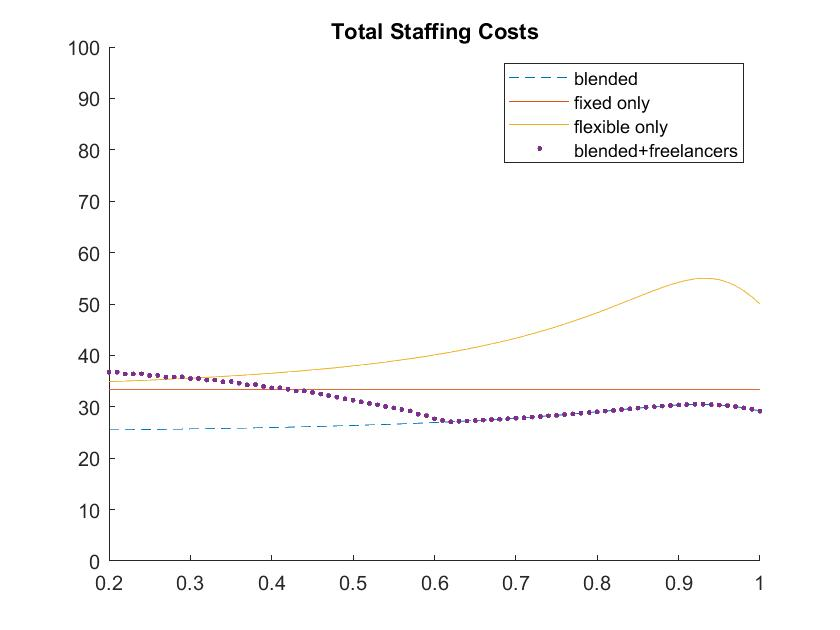
\includegraphics[height=4cm]{cost.jpg}
\caption{Total Staffing Costs}
\end{figure}
From the figure, we can see that the cost is lowest for the blended force, which grows closer to fixed cost as $q$ increases because we are employing more number of flexible workers to hedge the uncertainty.We can also see that the freelancers are adding an extra cost which is expected as we are employing freelancers for Quality of service but not cost reduction. Even with the added cost, the model with freelancers is cheaper when compared to just flexible or fixed when there is moderate to high uncertainty.
\end{frame}
\begin{frame}{Customer Perspective : Quality of Service}
\begin{figure}[hbt!]
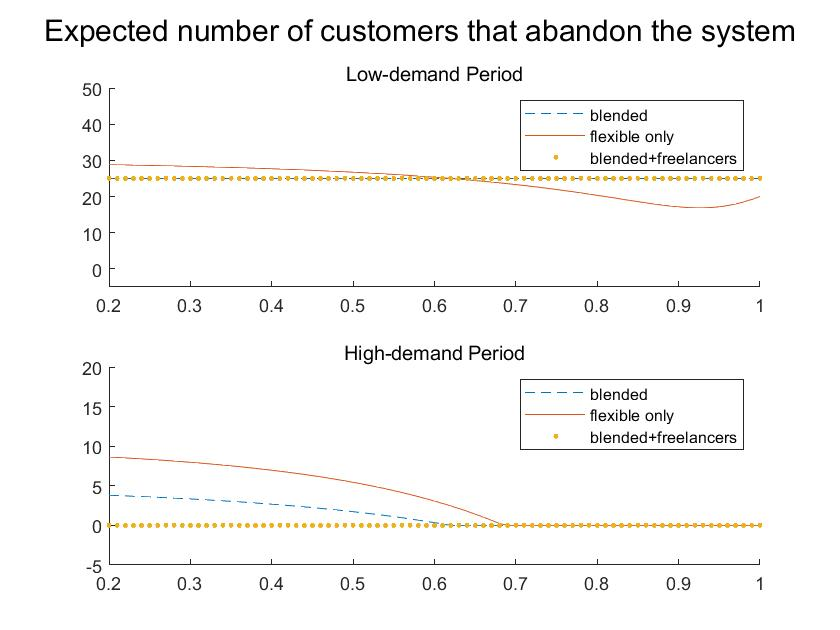
\includegraphics[height=5cm]{abandon.jpg}
\caption{Expected number of customers that abandon the system for p=0.8}
\end{figure}
We can see that in the low demand period that blended and blended+freelancer are the same as we are not employing any freelancers because the system is already overstaffed, and we can see that as the uncertainty increases we are over-staffing the system more and more hence increasing the quality but trading it off with the cost. 

\end{frame}
\begin{frame}{Customer Perspective : Quality of Service}
For the high demand period, employing freelancers is helping us in increasing in the quality of service when compared to  blended or just flexible. We can also see that as $q$ increases, we are over-staffing with flexible to hedge the uncertainty so we are not hiring any freelancers and the two plots merge. \bigskip

It is clear that the aim of adding freelancers is improving the quality of service by hedging against less show-up of flexible workers while trading off efficiency. When the show-up probability is as high as 0.8, we still see an improvement in quality of service with freelancers. We now explore the degree of improvement of quality of service for other show-up probabilities. We focus on the analysis of blended vs blended+freelancer regimes in the following sections.
\end{frame}
\begin{frame}{QoS when the show-up probability is high}
The previous figure represents this case. \bigskip

In the low-demand period, the number of flexible workers hired remains low, as a result, freelancers required to hedge the less show-up of flexible workers is very low (0 in this case). There is no improvement in the quality of service by adding freelancers but there is no loss in terms of efficiency because they are not being hired.\bigskip

In the high-demand period, we see a difference. Flexible workers would now be hired to supplement the fixed workforce. In the variability-dominated and a large part of the moderately uncertainty-dominated regimes, we see that the adding of freelancers improves the quality of service by reducing the number of customers abandoning the system. Once the value of $q$ exceeds 0.5, no freelancers are hired, and hence, there is no improvement in the quality of service. This happens because the manager hires high number of flexible workers because he knows that there is high variability in their show-up. Thus, the hiring of large number of flexible workers hedges the less show-up situation, and freelancers are not needed.
\end{frame}

\begin{frame}{QoS when the show-up probability is moderate}
We keep all the parameters same as the previous case but change the show-up probability, $p$, to $0.5$. \\
\begin{figure}[hbt!]
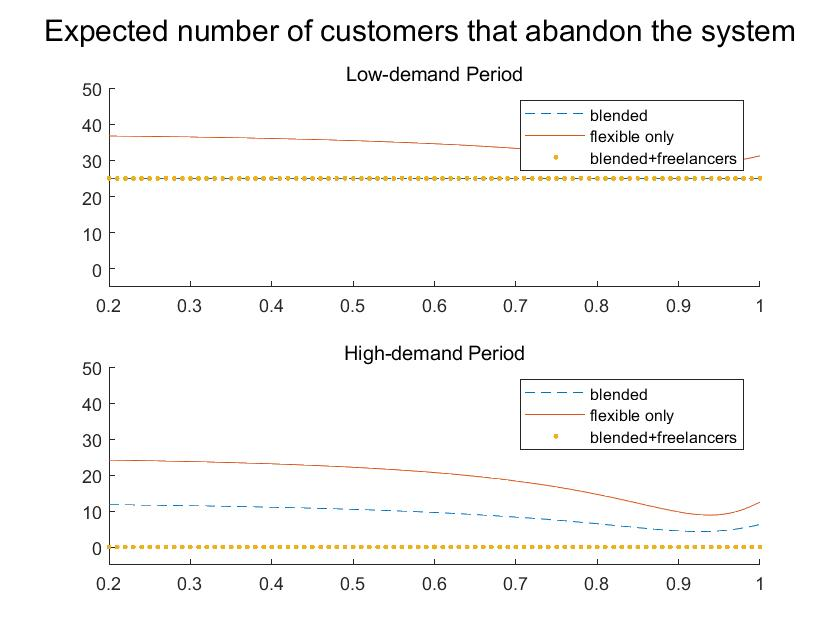
\includegraphics[height=5cm]{p0.5.jpg}
\caption{Expected number of customers that abandon the system for p=0.5}
\end{figure}
\end{frame}
\begin{frame}{QoS when the show-up probability is moderate}
In the low-demand period, the results are just like in the case of p=0.8. The number of flexible workers hired remains low, as a result, freelancers required to hedge the less show-up of flexible workers is very low (0 in this case). There is no improvement in the quality of service by adding freelancers but there is no loss in terms of efficiency because they are not being hired.\bigskip

In the high-demand period, we see a difference. Flexible workers would now be hired to supplement the fixed workforce. Across all regimes (from $q=0.2$ to $q=1$), we see that the adding of freelancers improves the quality of service by reducing the number of customers abandoning the system. 
\end{frame}

\begin{frame}{QoS when the show-up probability is low}
We keep all the parameters same as the previous case but change the show-up probability, $p$, to $0.2$. \\
\begin{figure}[hbt!]
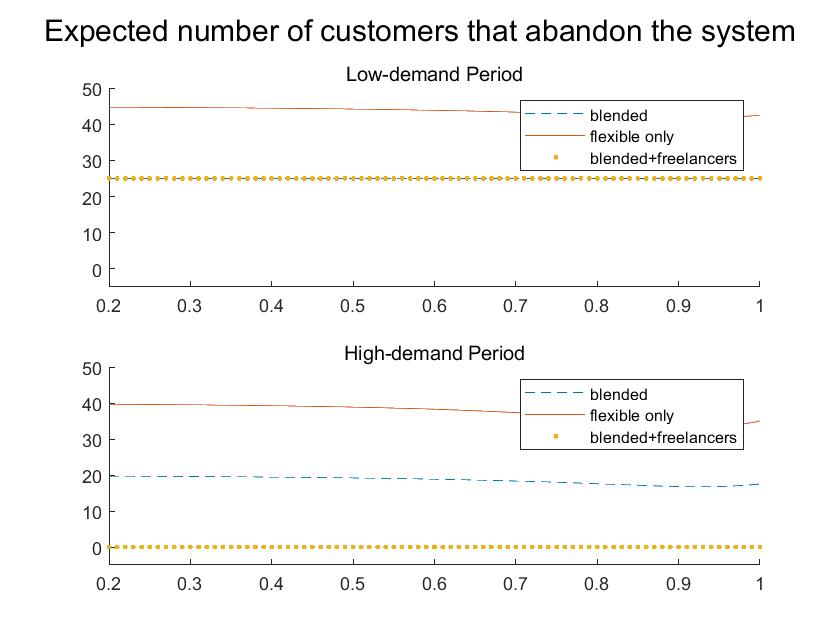
\includegraphics[height=5cm]{p0.2.jpg}
\caption{Expected number of customers that abandon the system for p=0.2}
\end{figure}
\end{frame}
\begin{frame}{QoS when the show-up probability is low}
In the low-demand period, the results continue to remain the same because the number of flexible workers hired remains low, and as a result, freelancers required to hedge the less show-up of flexible workers is very low.\bigskip

In the high-demand period, we see a trend very similar to the case when $p=0.5$. Across all regimes (from $q=0.2$ to $q=1$), we see that the adding of freelancers improves the quality of service by reducing the number of customers abandoning the system. The trend remains the same but the gap between the expected number of customers abandoning the system for the blended vs blended+freelancers case widens.
\end{frame}
  
\begin{frame}{Combining both perspectives}
In our addition to the model, we are more focused on improvement of quality of service, as we feel in real life, with the increased competition in the market, the emphasis has been shifting to quality of service. So, combining both the firm and customer perspective with an emphasis on quality of service, we can divide our model into mainly 3 regimens. \bigskip

\textbf{ \textit {(I) [Variability-dominated.]}} In this regime, we can see that the quality of service is best in the model with freelancers, but we can also see that the cost is very high and when we have high to moderate show-up probability for the flexible workers, the change in quality of service is not that substantial with the addition of freelancers, so for this regime, the best strategy would be to have a blended workforce without freelancers, when you have moderate to high show-up probabilities and only employ freelancers when you expect low probability of showing up. \bigksip

\textbf{ \textit {(II) [Moderately uncertainty-dominated.]}}
It is in this regime that we can see the workings of freelancers, the cost is lower with freelancers, when compared to just flexible or just fixed and though the cost is slightly higher when compared to blended, we can see that quality of service is greatly improved. So for this regime, the best strategy would be a blended+freelancer model. \bigskip

\textbf{ \textit {(III) [Strongly uncertainty-dominated.]}}
In this regime we are not employing any freelancers as we already hedge the uncertainty with a  high number of flexible workers and we can see that here we have almost the same cost for blended and fixed. In this case, we could see that blended is optimal.
\end{frame}

\section{Bibliography}
\begin{frame}{Bibliography}
    \bibliographystyle{plain}
\bibliography{demo}
\end{frame}
\end{document}

